\documentclass[a4paper, 10pt]{report}
\usepackage[T1]{fontenc}
\usepackage[utf8]{inputenc}
\usepackage[italian]{babel}
\usepackage{graphicx}

\usepackage{amsmath}
% \qed mette il simbolo a fine riga
% \qedsymbol lo mette subito dopo il punto 
\usepackage{amsthm}
\usepackage[T1]{fontenc}

\ttfamily

\title{Introduction to Progressively Finite Games}
\author{Romeo Rizzi}
\date{\today}

\newenvironment{esempio}{\begin{quote}\textbf{Esempio.} }{\end{quote}} 
\newenvironment{esercizio}{\begin{quote}\textbf{Esercizio.} }{\end{quote}}
\newenvironment{dimostrazione}{\textbf{Dimostrazione.} }{ \qed}
\newenvironment{dubbio}{\begin{quote}\textbf{Dubbio.} }{\end{quote}}


\theoremstyle{definition} % plain, break, marginbreak, changebreak, change, margin%
\newtheorem{theorem}{Teorema}
\newtheorem{lemma}{Lemma}
\newtheorem{definizione}{Definizione}
\newtheorem*{definizioneDoc}{Definizione}
\newtheorem*{definizioneInformale}{Definizione Informale}
\newtheorem*{definizioneFormale}{Definizione Formale}
\newtheorem{algorithm}{Algoritmo}

\begin{document}

\maketitle
\newpage
\begin{center}
\section*{Progressively finite games}
\end{center}


Il presente documento tratta di una particolare classe di giochi combinatorici
a due giocatori, comunemente chiamati progressively finite games. 
Ai fini della nostra analisi, definiremo un \emph{progressively finite game} come un
qualsiasi gioco che possa essere visualizzato come un grafo diretto aciclico e
finito, nel quale i giocatori percorrono a turno un arco del grafo. Se il
giocatore che deve muovere non trova archi uscenti dal nodo corrente, perder\`a
la partita. Nel corso dell'analisi, si supporr\`a che entrambi i giocatori
scelgano la migliore mossa a loro disposizione. 


\begin{esempio}
Due giocatori, $A$ e $B$, avendo a disposizione solo monete da $1$ e da $2$ Euro,
dovranno a turno metterne una in un piatto, inizialmente vuoto, che pu\`o
contenere al pi\`u $10$ Euro. Quando questo sar\`a pieno, il gioco terminer\`a
con la vittoria del giocatore che ha messo l'ultima moneta. 
\end{esempio}

Dopo aver giocato diverse partite, ci si render\`a conto che, nell'ipotesi di
gioco ottimo, il giocatore che d\`a inizio al gioco vince sempre. 
Questo fatto \`e maggiormente visibile  modellando il gioco con un grafo 
orientato, in modo tale che ogni suo vertice corrisponda ad una posizione 
possibile del gioco, e ogni suo arco rappresenti una possibile mossa 
da una posizione ad un'altra.
Il grafo del gioco considerato \`e quello in Figura~\ref{game_1_2coins}.

\begin{figure}[h]
  \label{game_1_2coins}
  \centerline{
    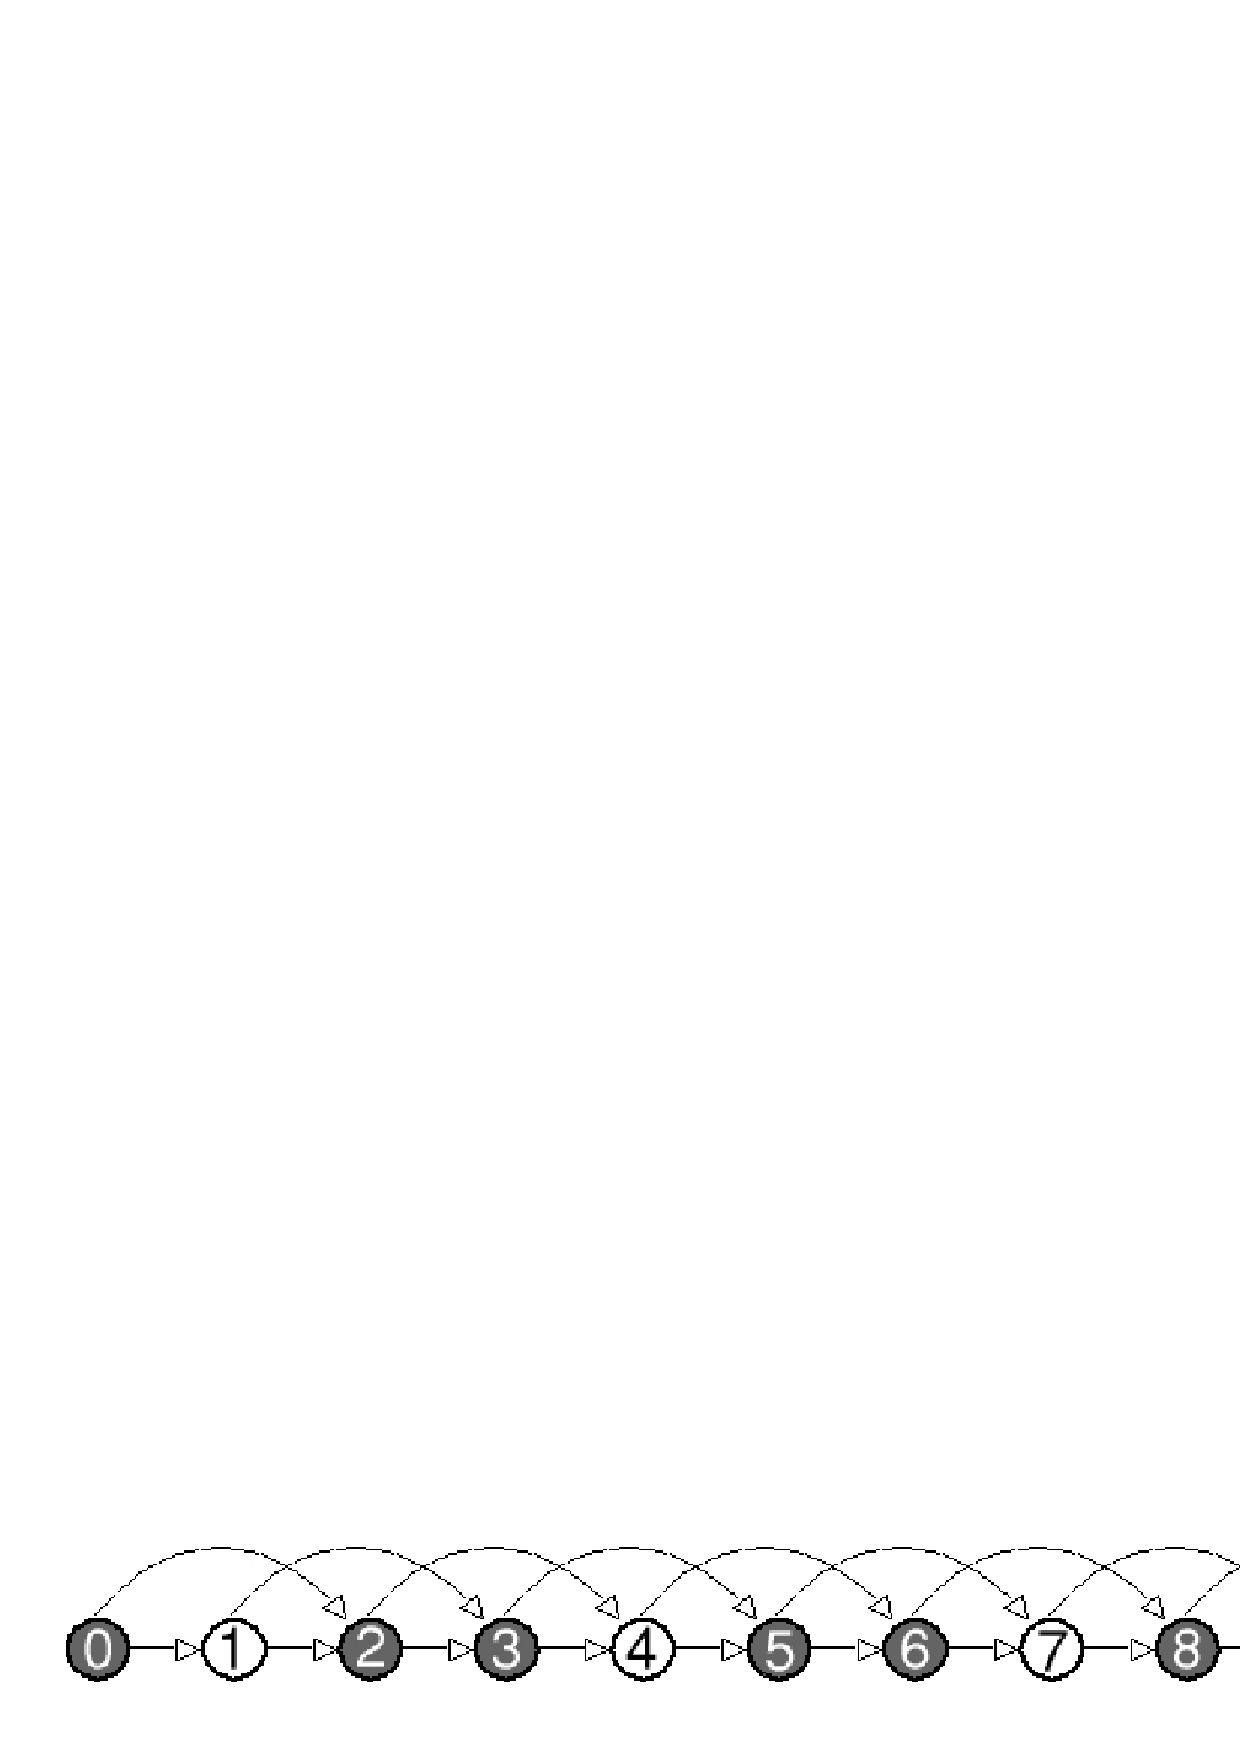
\includegraphics[width=0.96\textwidth]{figs/game_1_2coins.png}
  }
  \caption{\textsl{Gioco delle monete.}}
\end{figure}

La strategia vincente (in questo caso unica) consiste nel porsi sempre in un nodo
con etichetta $x$ tale che $10-x \equiv 0 \mod 3$.
Il giocatore che arriva sull'ultimo vertice del grafo, quello con il numero~$10$,
vince la partita, poich\'e tale vertice \`e un pozzo e perci\`o l'altro
giocatore non ha pi\`u alcuna mossa a disposizione.

Se \emph{pozzo} ti \`e un termine nuovo, e se non avevi mai incotrato
propriet\`a dei grafi diretti e aciclici quali, ad esempio, la presenza
necessaria di pozzi, ti suggeriamo di esplorare l'Appendice~\ref{app_a}, prima
di avventurarti nella teoria dei progressively finite games. Nell'appendice
potrai trovare anche alcune definizioni, che ti saranno utili per comprendere
meglio questa classe di giochi e confrontarti con la terminologia da noi
adottata.
\newline

Il nostro scopo \`e individuare una strategia vincente, ossia una serie di
mosse tali da portare un giocatore alla vittoria comunque giochi
l'avversario. Ovviamente, solo uno dei due giocatori potr\`a avere una
strategia vincente.
\newline

\begin{esercizio}
L' ``ovviamente'', nella frase di cui sopra, nasconde delle insidie. Infatti,
per dimostrare ciò in modo informale, dovremmo per prima cosa fornire una
nozione precisa di strategia vincente. Prova a fornirne una tu e poi controlla
se essa corrisponde con quella da noi proposta qui sotto.
\end{esercizio}

\begin{definizioneInformale}[Strategia vincente]
Dire che un giocatore ha una strategia vincente significa affermare che,
giocando in modo ottimo, egli \`e sempre in grado di aggiudicarsi la partita,
trovando una contromossa per ogni possibile mossa dell'avversario.
\end{definizioneInformale}

Si noti ora come, in base alla nostra nozione ``informale'' di cui sopra, il
fatto che il giocatore di turno possieda o meno una strategia vincente
\textbf{non} dipende da come il giocatore conduca la partita (abbiamo fatto
l'ipotesi di gioco ottimo), bens\`i dipende solamente dalla posizione (nodo
del grafo) in cui ci si trova.

I nodi del grafo sono pertanto partizionati in due insiemi:
\begin{itemize}
\item L'insieme dei nodi in cui esiste una strategia vincente (nodi
  chi-tocca-vince);
\item L'insieme dei nodi in cui non esiste alcuna strategia vincente (nodi
  chi-tocca-perde).
\end{itemize}


\begin{definizioneFormale}[Strategia vincente]
Una data posizione (nodo del grafo) ammette una strategia vincente se offre
una mossa che conduce ad una posizione ``chi-tocca-perde''. Una posizione \`e
di tipo ``chi-tocca-perde'' se non ammette una strategia vincente.
\end{definizioneFormale}

\begin{dubbio}
Siete convinti della validit\`a della definizione di cui sopra? Un pericolo
\`e evidente: si \`e definito il concetto di strategia vincente in
termini di posizioni ``chi-tocca-perde'', e viceversa. Il classico cane che si
morde la coda! Questa situazione \`e rappresentata con un ciclo diretto in
Figura~\ref{winning_strategy_kicks_back_to_kernel}.
\end{dubbio}

\begin{figure}[h]
  \label{winning_strategy_kicks_back_to_kernel}
  \centerline{
    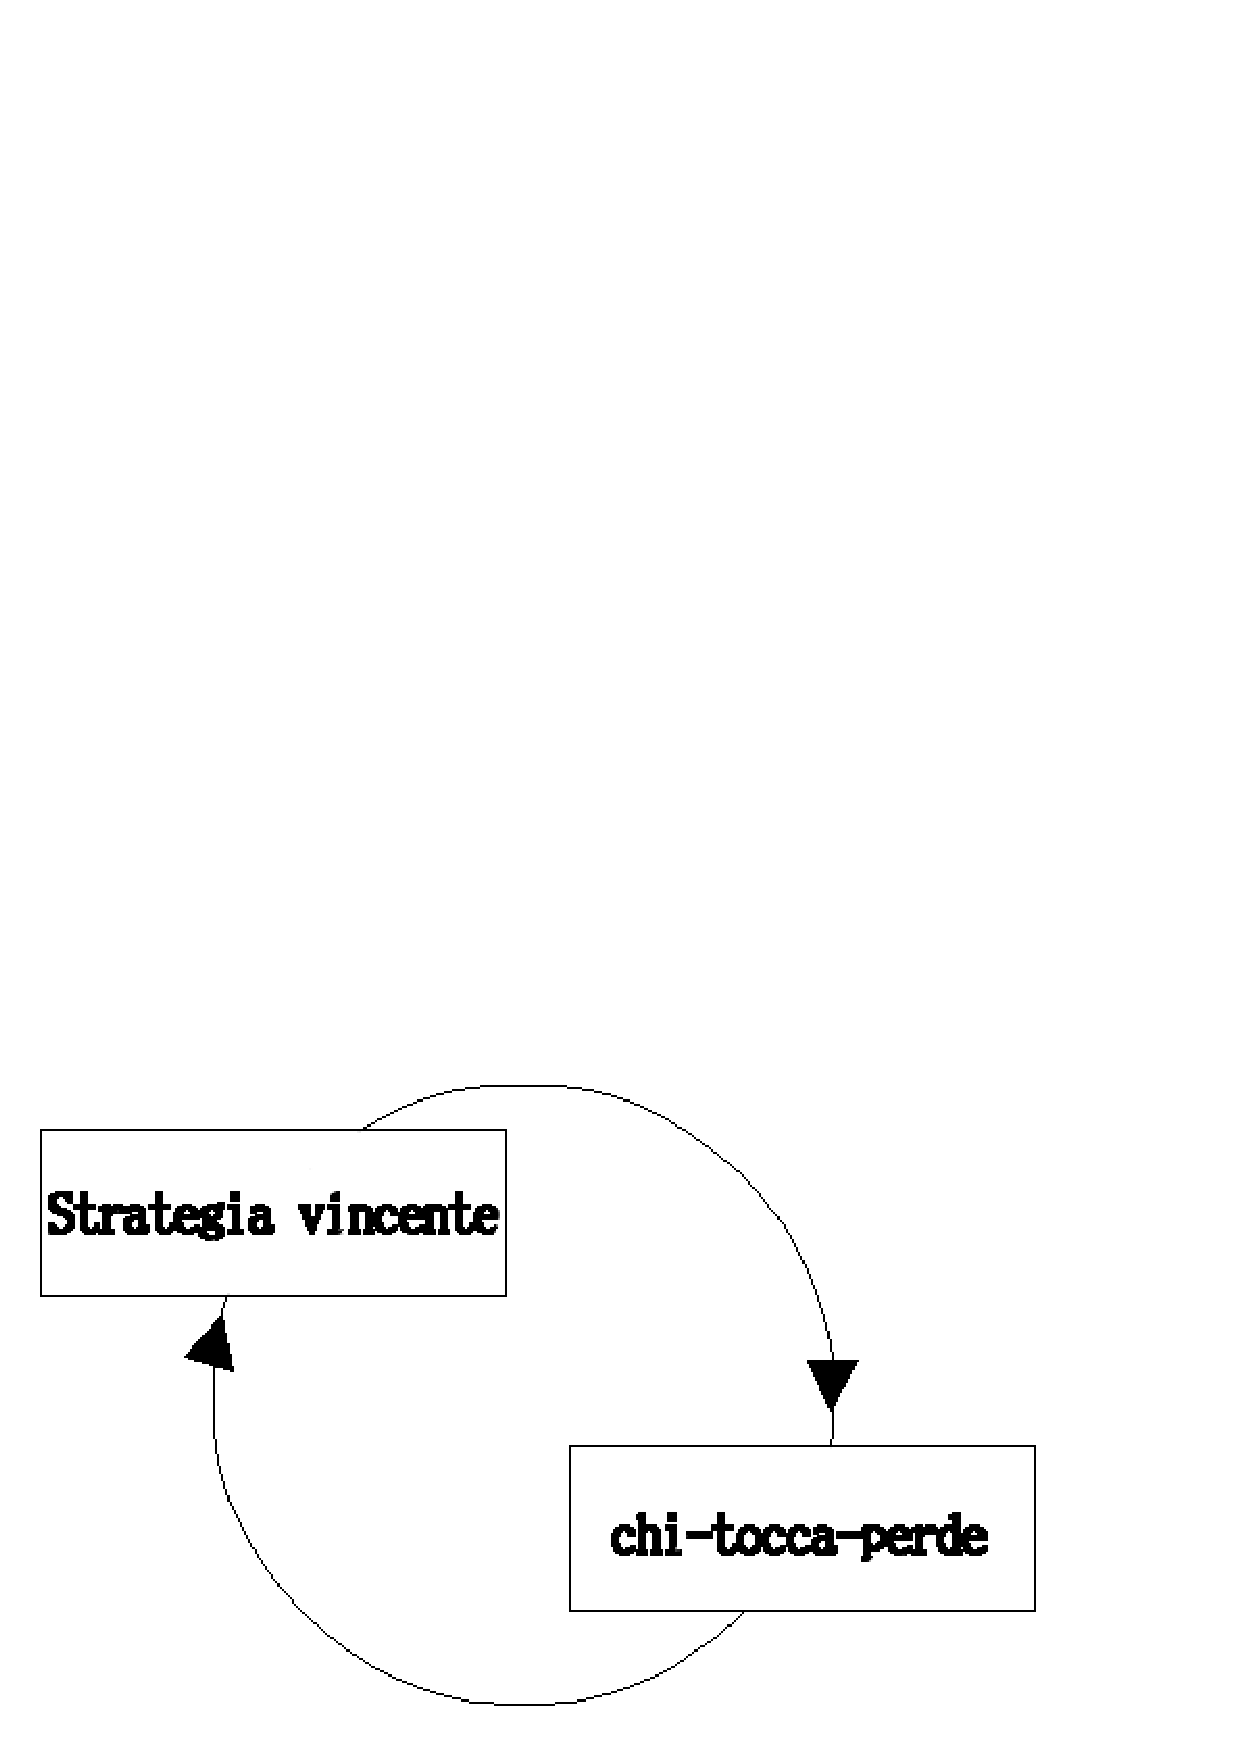
\includegraphics[width=0.5\textwidth]{figs/winning_strategy_kicks_back_to_kernel.png}
  }
  \caption{\textsl{Schema ciclico delle definizioni.}}
\end{figure}

Anche se un primo dubbio \`e pertanto legittimo, possiamo tuttavia dire che, la
definizione data sopra, sebbene ricorsiva, risulta inequivocabile, poich\'e il
grafo che rappresenta il gioco \`e aciclico; saranno pertanto i pozzi del
grafo ad offrire un punto di partenza, o base, alla definizione stessa.

\begin{esempio}
Nel gioco delle monete, un pozzo \`e rappresentato dal nodo 10. Il
giocatore di turno non ha una mossa valida e quindi, in base alla definizione
(formale), non ha una strategia vincente. Ne segue che 10 \`e una posizione
``chi-tocca-perde''. Quindi 9 ammette una strategia vincente, vista la
presenza di un arco da 9 a 10. Lo stesso dicasi per 8. Di 7 possiamo
nuovamente dire che esso rappresenta una posizione ``chi-tocca-perde'',
poich\'e non offre una strategia vicente, visto che non vi sono archi uscenti
verso nodi ``chi-tocca-perde''; e cos\`i via per gli altri nodi. 
In questo gioco, tutte le posizioni ``chi-tocca-perde'' sono rappresentate dai
vertici colorati di bianco in Figura~\ref{game_1_2coins}.
\end{esempio}

Prima di approfondire la teoria dei progressively finite games, vorrai forse
sperimentare quanti e quali giochi ricadono in questa categoria. 

\begin{enumerate}
\item[\textbf{Esercizio 1.}]   Data una scacchiera di 8x8 caselle, due
  giocatori devono muovere a turno un cavallo, seguendo le regole previste dal
  gioco degli scacchi. Il cavallo, partendo da una posizione fissata a priori,
  non deve mai tornare su una casella in cui \`e gi\`a stato. Quando un
  giocatore non ha pi\`u mosse a disposizione, perde la partita. Si invita il
  lettore a verificare che questo gioco rientra nella categoria dei
  progressively finite games. Riesci a disegnare il grafo che modella questo
  gioco? Quali difficolt\`a hai incontrato nel fare ci\`o? 
\item[\textbf{Esercizio 2.}] Una scacchiera di 5x5 caselle viene coperta con
  delle monete, una per casella, in modo tale da formare un quadrato composto
  da 25 monete. A turno, due giocatori prendono un qualsiasi gruppo di
  monete, purch\'e il primo giocatore ne prelevi una fila (o parte di una
  fila) in orizzontale, mentre il secondo giocatore compia la sua mossa
  prelevando una fila (o parte di una fila) posta verticalmente. Il gioco
  termina nel momento in cui non ci sono pi\`u monete sulla scacchiera. Il
  giocatore che ha prelevato l'ultimo gruppo di monete vince la
  partita. Sapresti disegnare il grafo che modella questo gioco? E sei in
  grado di individuare una strategia vincente?
\item[\textbf{Esercizio 3.}] Nel corso di una partita a scacchi il bianco si
  trova in una situazione di grande difficolt\`a: il nero ha la possibilit\`a
  di concludere la partita con uno scacco matto forzato in 5 mosse. Vista la
  situazione favorevole, il nero considera persa la partita se non riesce a
  vincere nel corso delle 5 mosse successive. Possiamo dire, a questo punto,
  di essere in presenza di un progressively finite game?
\item[\textbf{Esercizio 4.}] Inventa tu un gioco che rientri nella categoria
  dei progressively finite games. Dei giochi che gi\`a conosci, sai
  individuarne qualcuno che ricade in questa categoria? Riguardo ai tuoi
  giochi combinatorici preferiti, sapresti proporre delle modifiche alle
  regole che riducano il gioco ad un progressively finite game?

\end{enumerate}


\begin{center}
\subsection*{Kernel}
\end{center}

Un \textbf{kernel} in un grafo \`e un insieme di vertici con le seguenti 
propriet\`a:
\begin{itemize}
\item[(i)] Non ci sono archi che congiungono due vertici nel kernel;
\item[(ii)] Ogni vertice che non \`e nel kernel ha almeno un successore nel kernel.
\end{itemize}

Nel gioco in Figura~\ref{game_1_2coins} il kernel \`e formato dai vertici 1, 4, 7, 10.

Non tutti i grafi hanno un kernel. Si consideri ad esempio il grafo in Figura~\ref{no_kernel}. 

\begin{figure}[h]
  \label{no_kernel}
  \centerline{
    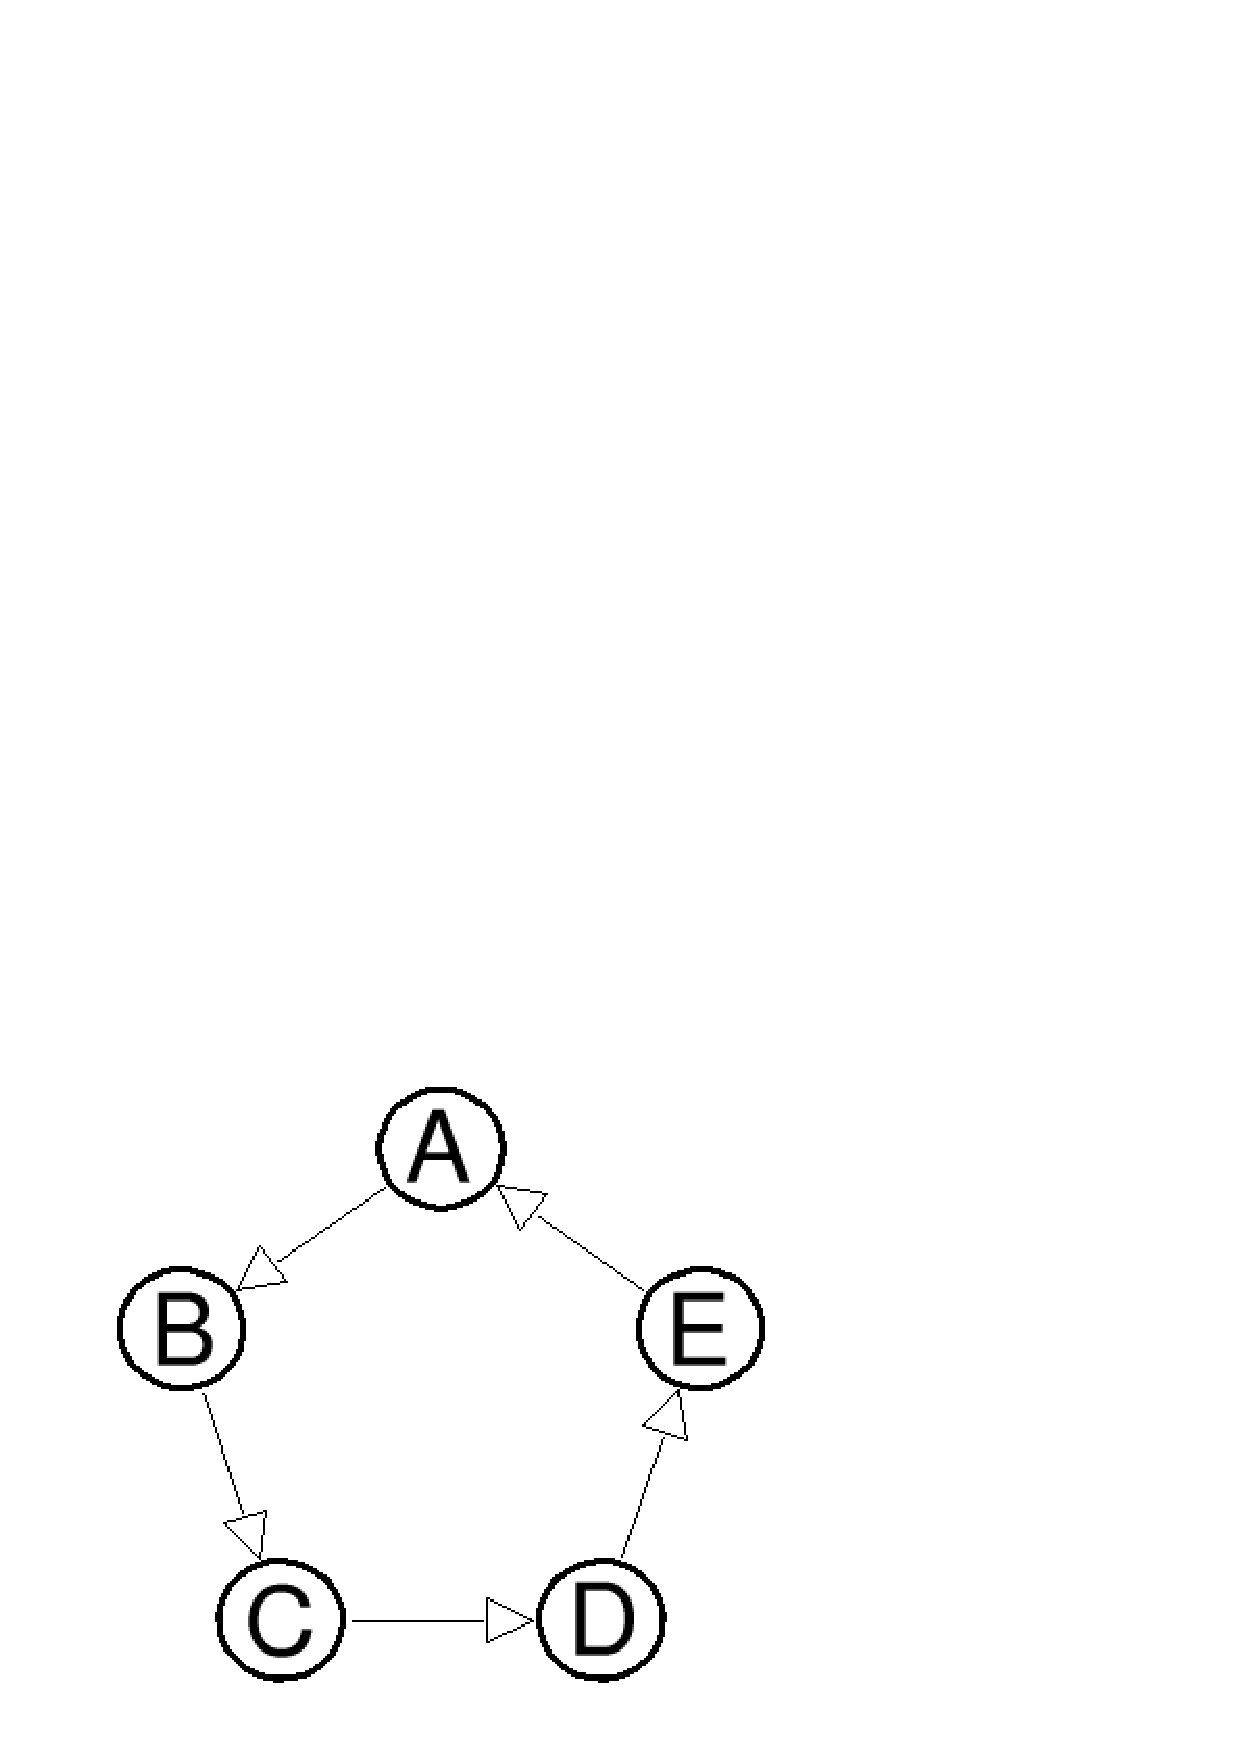
\includegraphics[width=0.5\textwidth]{figs/no_kernel.png}  
  }
  \caption{\textsl{Esempio di grafo che non ammette kernel.}}
\end{figure}

Per simmetria si pu\`o assumere che, se il grafo ammettesse un kernel K, il 
vertice $a$ ne farebbe parte. Quindi $b \not\in K$ per (i), $c \in K$ per (ii),
$d \not\in K$ per (i), $e \in K$ per (ii), allora $a \not\in K$ per (i)
- assurdo!
\newline

\begin{theorem}
Se $G$ \`e il grafo di un progressively finite game, allora $G$ ha
un kernel ed esso \`e unico.
\end{theorem}

\begin{dimostrazione}
Preso il grafo $G$, consideriamo un suo pozzo $p$. Il Lemma~\ref{pozzo} (vedi
Appendice~\ref{app_a}) ne garantisce l'esistenza. 
Sia $G'$ il grafo ottenuto da $G$ eliminando $p$ e tutti i vertici in
$N(p)$. Si  noti che $G'$ \`e un grafo diretto aciclico e finito pi\`u piccolo
di $G$.  Per induzione, $G'$ ha un kernel $K'$. Dimostreremo che $K = K' \cup
\{p\}$ \`e un kernel di $G$. La propriet\`a (i) del kernel \`e verificata,
poich\'e nessun vertice appartenente a $K'$ pu\`o essere adiacente a $p$.
La propriet\`a (ii) \`e soddisfatta poich\'e tutti i vertici in $N(p)$ hanno
un arco uscente verso $p$, e $p$ \`e in $K$.
Per l'unicit\`a, si consideri un generico kernel $H$ di $G$. Si noti che $p
\in H$, poich\`e, se cos\`i non fosse, $p$, per la propriet\`a (ii) del
kernel, dovrebbe avere un arco uscente verso un vertice nel kernel - ma $p$
\`e un pozzo. Si noti anche che $N(p) \cap H = \emptyset$ (per la propriet\'a
(i) del kernel). Da questo segue che $H - \{p\}$ \`e un kernel per $G'$.
Poich\'e $G'$ \`e pi\`u piccolo di $G$, per induzione ha un unico kernel,
quindi $K' = H -\{p\}$. Siccome $K = K' \cup \{p\}$, ne segue che $K = H$.
\end{dimostrazione}
\newline

\begin{theorem}
In un progressively finite game, una strategia vincente consiste nel muovere ad
ogni turno nei vertici del kernel.
\end{theorem}

\begin{dimostrazione}
Per la propriet\`a (i) del kernel, se il primo giocatore muove su un vertice 
del kernel, il secondo giocatore dovr\`a necessariamente muovere su un vertice 
che non \`e nel kernel. Per la propriet\`a (ii), il primo giocatore, quindi, 
potr\`a sempre muovere in un vertice nel kernel da un vertice che non \`e nel 
kernel. Poich\`e il gioco deve terminare e i pozzi si trovano tutti 
nel kernel, il primo giocatore si aggiudicher\'a la partita.
\end{dimostrazione}
\newline

I teoremi visti sopra sono costruttivi; dato un grafo diretto \`e possibile
trovarne il kernel in tempo lineare.

\newpage

\begin{algorithm} \label{findkernel}
Sia $G$ un grafo aciclico e $V$ l'insieme dei suoi vertici e $p$ un generico
pozzo.
\end{algorithm}

\begin{minipage}{8cm}
{\small \sf
Find\_Kernel(G)\newline
    if |V| = 1 then return V;\newline
    else return \{p\} $\cup$ Find\_Kernel(G\char92N(p)\char92{p}).
}
\newline

\end{minipage}

\begin{enumerate}
\item [\textbf{Esercizio 5.}] Prova a implementare l'Algoritmo~\ref{findkernel}
  e a verificare che \`e lineare.
\end{enumerate}

In base all'Algoritmo~\ref{findkernel}, sembrerebbe che non ci sia alcuna
difficolt\`a nell'individuare una strategia vincente in un qualsiasi
progressively finite game. L'Algoritmo~\ref{findkernel} \`e infatti lineare
(meglio non si pu\`o!) nelle dimensioni del grafo associato al progressively
finite game. 
Tuttavia, il generico gioco nella classe dei progressively finite game, non
viene descritto in termini del grafo diretto da noi ad esso associato, ma
fornendo un ambiente e delle regole di gioco che possono notevolmente variare.

All'interno di questa formulazione pi\`u colorita (piatto con gli Euro,
cavallo sulla scacchiera), compaiono inoltre dei parametri (numero di
\textbf{10} Euro, \textbf{dimensione} della scacchiera). 

Una volta scelto il gioco di nostro interesse, la dimensione del grafo
associato \`e spesso esponenziale nel parametro; era questo, ad esempio, il
problema riscontrato nell'Esercizio 2.

Per meglio illustrare questo problema, e scoprire come talvolta esso possa
essere superato, considereremo il gioco del Nim, ed introdurremo il concetto
di somma di giochi e le Grundy functions. 


\begin{center}
\section*{Nim}
\end{center}

Il Nim \`e probabilmente uno dei giochi pi\`u antichi e impegnativi che
rientra nella categoria dei progressively finite games. Nato probabilmente in
Cina, nella sua versione pi\`u popolare, ci sono 12 monete distribuite su tre
righe come riportato in Figura~\ref{nim_game}.

\begin{figure}[h]
  \label{nim_game}
  \centerline{
    \fbox{
       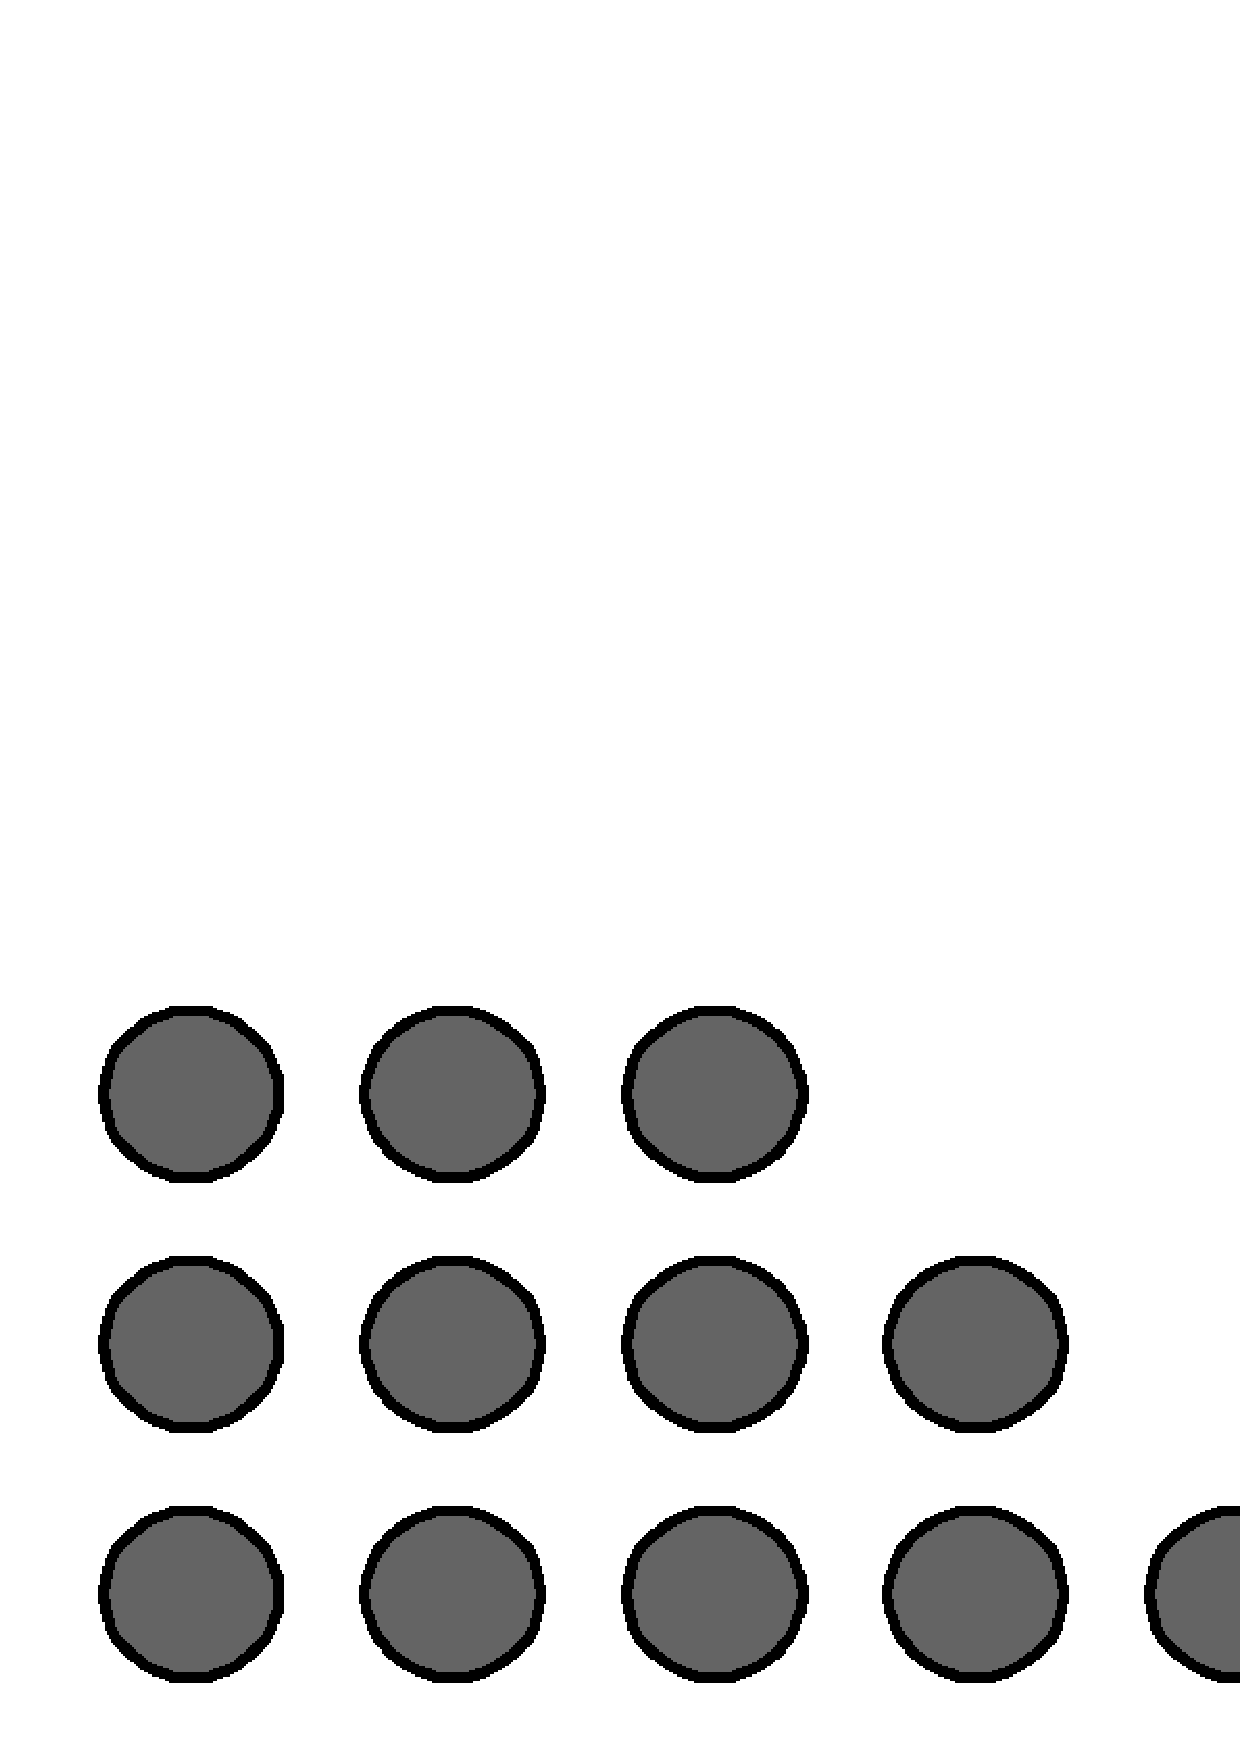
\includegraphics[width=0.5\textwidth]{figs/nim_game.png}  
    }
  }
  \caption{\textsl{Versione comune del Nim.}}
\end{figure}

Le regole del gioco sono piuttosto semplici: a turno, i due giocatori,
pre\-levano una o pi\`u monete adiacenti da una riga a scelta, partendo sempre
da uno degli estremi; il giocatore che prende l'ultima moneta vince.
Si invita il lettore a provare che la strategia vincente, per il primo
giocatore, consiste nel prendere due monete dalla riga superiore.

Il gioco pu\`o comunque essere generalizzato ad un numero qualsiasi di righe
contenenti un numero qualsiasi di monete.
Nonostante una strategia vincente sia nota ai matematici, questa non \`e
semplice e di immediata comprensione. Di fatto, molte persone continuano a
giocare con interesse questo gioco. Un'altra versione molto comune ha 4 righe,
la prima con una sola moneta, la seconda con 2, la terza con 3 e la quarta
con 4, come mostra la Figura~\ref{nim_sticks}, dove abbiamo preferito utilizzare
bastoncini in quanto eravamo a corto di monete.

\begin{figure}[h]
  \label{nim_sticks}
  \centerline{
       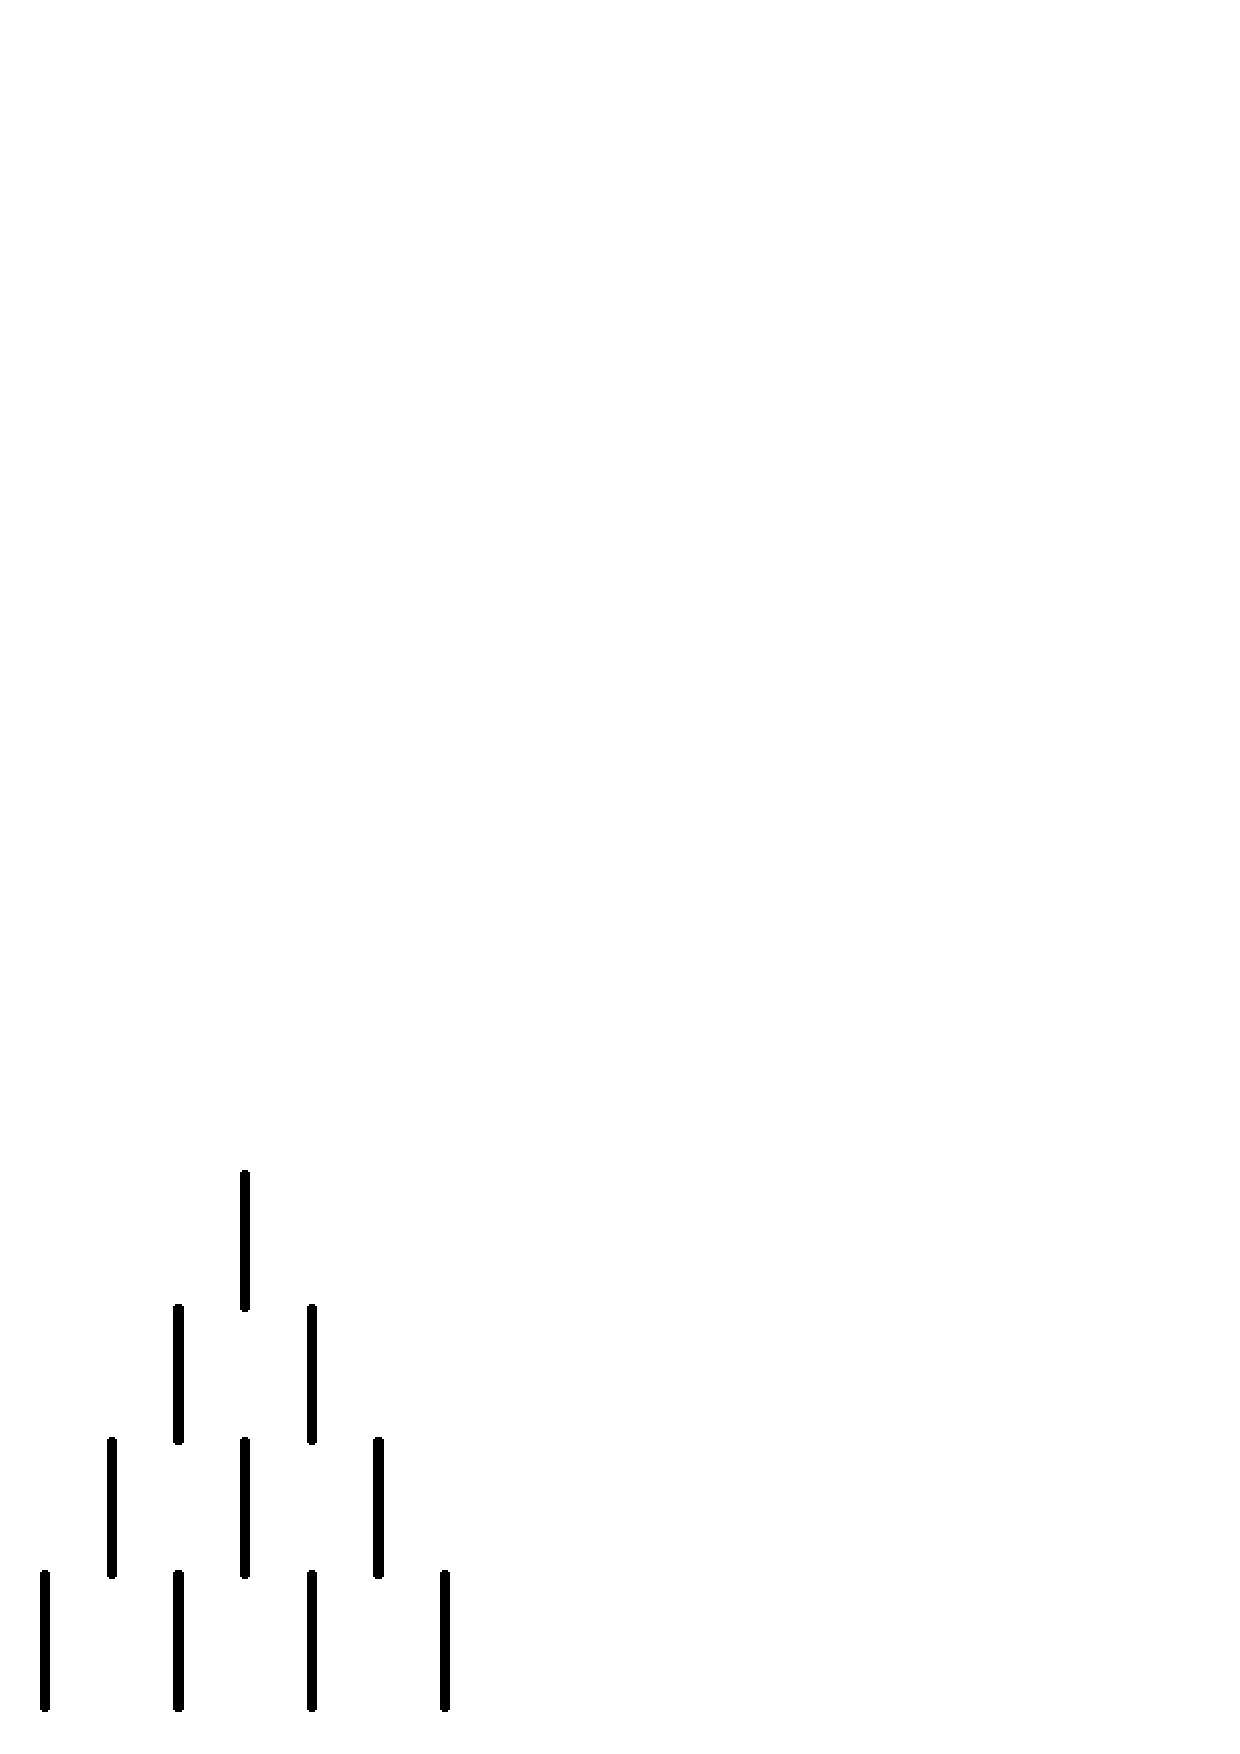
\includegraphics[width=0.3\textwidth]{figs/nim_sticks.png}  
  }
  \caption{\textsl{Altra comune versione del Nim.}}
\end{figure}

Qualsiasi sia la versione del gioco preferita, e qualsiasi sia la posizione
attuale, se c'\`e una sola riga la strategia vincente \`e ovvia, e consiste
nell'eliminarla tutta. Se per esempio tale riga \`e formata da 3 monete, il
grafo del gioco \`e quello in Figura~\ref{nim_1stack}.

\begin{figure}[h]
    \label{nim_1stack}
    \centerline{
       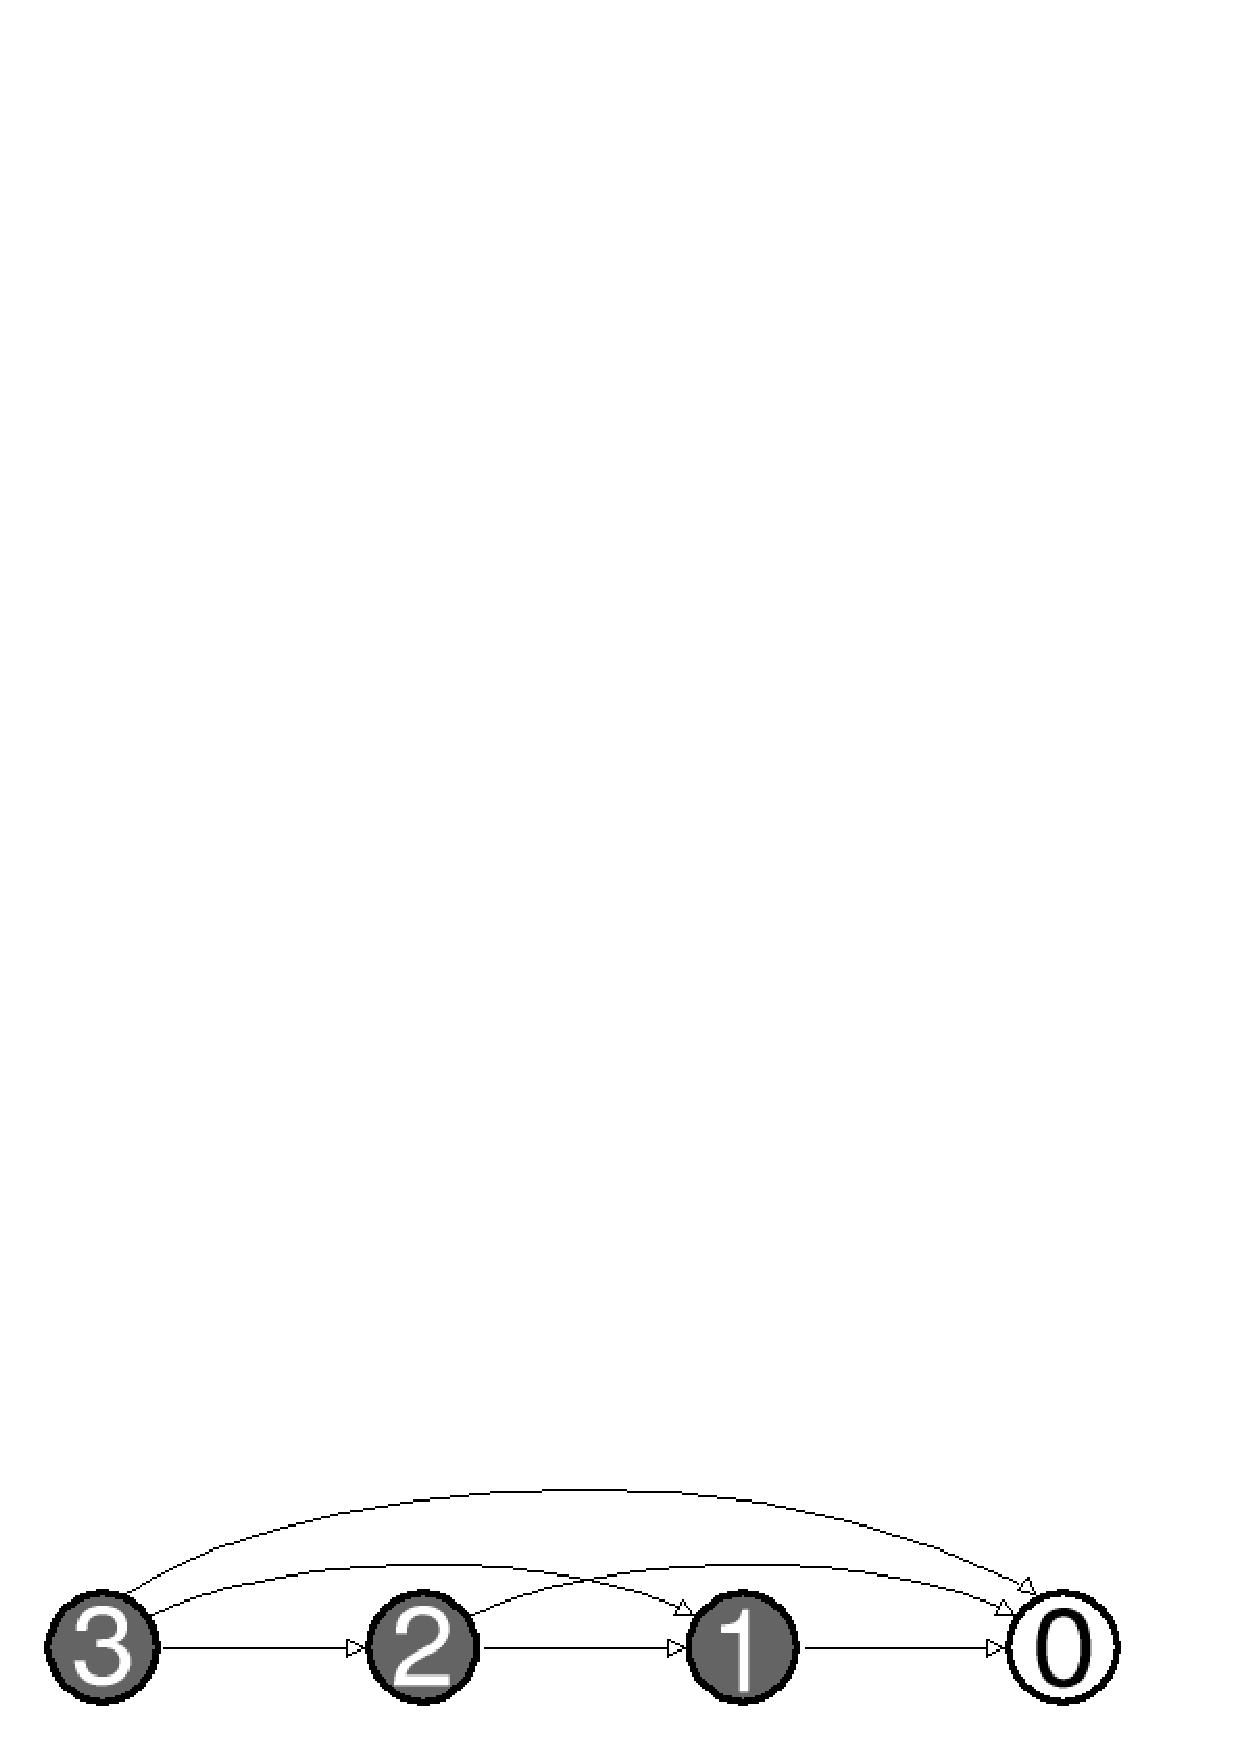
\includegraphics[width=0.5\textwidth]{figs/nim_1stack.png}  
    }
    \caption{\textsl{Nim su una sola pila di 3 monete.}}
\end{figure}

Aumentando il numero delle righe, la dimensione del grafo aumenta in modo
esponenziale, poich\'e il grafo di un Nim su $k$ righe corrisponde alla
somma diretta (vedi Appendice~\ref{app_a}) dei grafi di ciascuna delle $k$
righe prese singolarmente.  

Ad esempio, il gioco del Nim formato semplicemente da due righe composte da
due sole monete ciascuna, \`e mostrato in Figura~\ref{nim2of2}.

\begin{figure}[h]
  \label{nim2of2}
  \centerline{
       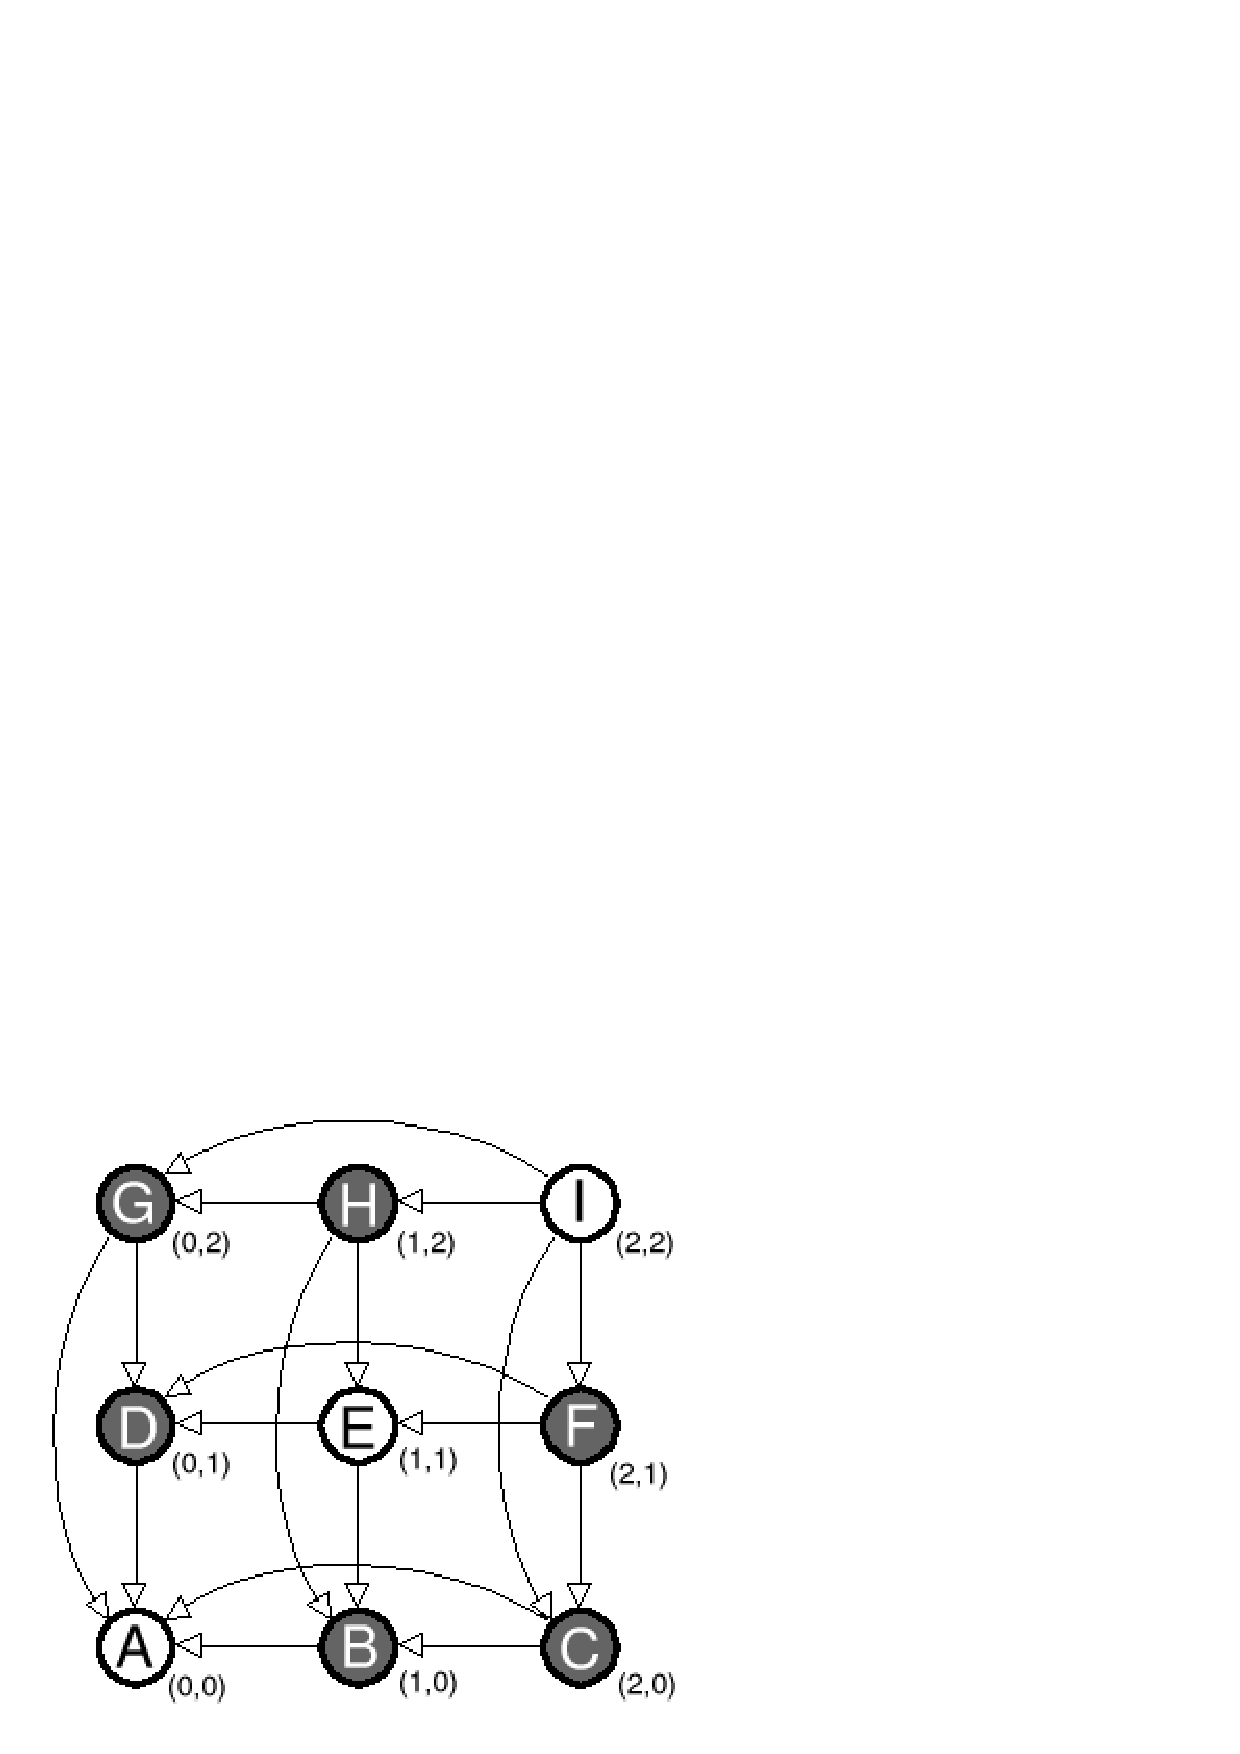
\includegraphics[width=0.7\textwidth]{figs/nim2of2.png}  
  }
  \caption{\textsl{Grafo del Nim con $2$ pile da $2$ monete ciascuna.}}
\end{figure}


\subsection*{Grundy Function}

L'aumentare di complessit\`a del gioco rende necessaria l'introduzione di un
concetto pi\`u robusto rispetto a quello di kernel.
\newline
\begin{definizioneDoc}[Grundy function]  
Una Grundy function $g(x)$ \`e una funzione che associa, ad ogni
vertice $x$ del grafo $G$, il pi\`u piccolo intero non negativo che non
\`e stato assegnato ad alcuno dei successori di $x$.
\end{definizioneDoc}

Ogni DAG ammette una Grundy function, ed essa può essere univocamente costruita in modo analogo a quanto abbiamo visto per il kernel.
Poich\'e i pozzi non hanno successori, questi avranno Grundy number 0 (il
pi\`u piccolo intero non negativo). Quindi, ricorsivamente, si determina $g(x)$
prima per i vertici $v \in N(p)$, quindi per i vertici in $N(v)$, e cos\`i
via. In pratica, ad ogni passo, possiamo determinare il valore della Grundy
function per quei nodi $x$ che sono pozzi nel grafo ottenuto da $G$
rimuovendo $p$ ed $N(p)$.
Cos\`i facendo, tutti i vertici di cui $x$ \`e successore, vengono processati
prima di determinare il Grundy number di $x$.

Come esempio, costruiremo la Grundy function sul gioco delle monete nel
piatto. Per prima cosa, assegnamo Grundy number 0 a tutti i pozzi, quindi
passiamo ai vertici adiacenti. Consideriamo prima quello numerato con
9. Poich\'e al suo successore \`e stato assegnato Grundy number 0, a 9 verr\`a
assegnato il valore 1. Consideriamo ora il vertice numerato con 8. Poich\'e i
suoi due successori sono numerati con 0 ed 1, a lui assegnamo Grundy number
2. Al vertice 7 assegnamo Grundy number 0, poich\'e i suoi archi escono verso
vertici i cui Grundy number sono 1 e 2; e cos\`i via per tutti gli altri
vertici.
\newline

Abbiamo visto che il kernel esiste ed \`e unico. Possiamo ora meglio
individuarne i nodi in termini della Grundy function.

\begin{lemma}
Tutti e soli i vertici che hanno Grundy number 0 sono vertici del kernel.
\end{lemma}

\begin{dimostrazione}
Dalla definizione di Grundy function, un vertice $x$, con
Grundy number 0, non pu\`o avere un arco uscente verso un altro vertice con
Grundy number 0; altrimenti non sarebbe stato possibile etichettarlo con 0. In
modo analogo, un vertice $y$, con Grundy number $k>0$, deve avere un arco
verso un vertice con Grundy number 0, altrimenti $y$ sarebbe etichettato con 0.
I vertici con Grundy number 0 soddisfano, pertanto, entrambe le propriet\`a del
kernel.
\end{dimostrazione}
\newline

Mostreremo ora come calcolare il Grundy number di un vertice, in una somma
diretta di grafi, partendo dai  Grundy number dei singoli vertici di ogni
grafo. Tale calcolo viene chiamato \emph{somma digitale}.
\newline
La somma digitale $c$ degli interi non negativi $c_1, c_2, \ldots, c_n$
si scrive:
\begin{center}
  $c=c_1 \dot{+} c_2, \dot{+} \ldots \dot{+} c_n$
\end{center}

Per calcolarla bisogna convertire in notazione binaria ogni numero $c_i$ con
$1 \le i \le n$;
\begin{center}
$c_i = c_{i}^{(0)}\cdot 2^0 + c_{i}^{(1)}\cdot 2^1 + c_{i}^{(2)}\cdot 2^2 +
  \ldots + c_{i}^{(n)}\cdot 2^n$
\end{center}
A questo punto $c^{(k)}$, ossia la $k$-esima cifra binaria che compone il 
numero $c$, si calcola attraverso il seguente:
 $c^{(k)}=c_{1}^{(k)}+c_{2}^{(k)}+ \ldots +
c_{n}^{(k)}$ $(mod 2)$.\\

Ad esempio, la somma digitale per i numeri 3, 5, 8, 13, 15 \`e mostrata nella
seguente tabella:
{\small
\begin{center}
  \mbox{
    \begin{tabular}[b]{rccccl}
          & $2^3$ & $2^2$ & $2^1$ & $2^0$ &   \\
      \hline
      3=  &   0   &   0   &   1   &   1   & + \\
      5=  &   0   &   1   &   0   &   1   & + \\
      8=  &   1   &   0   &   0   &   0   & + \\
      13= &   1   &   1   &   0   &   1   & + \\
      15= &   1   &   1   &   1   &   1   & = \\
      \hline
          &   1   &   1   &   0   &   0   & =12
    \end{tabular}
  }
\end{center}
}
\begin{theorem}
Se i grafi $G_1$ e $G_2$ hanno rispettivamente Grundy function $g_1(x)$ e
$g_2(x)$ allora il grafo $G = G_1 + G_2$ ammette Grundy function $g(x)$
definita come segue: 
\begin{equation}
  g(x) = g((x_1, x_2)) := g_1(x_1) \dot{+} g_2(x_2).
\end{equation}
\end{theorem}

\subsubsection*{Dimostrazione}
Dobbiamo mostrare che, per ogni nodo $x = (x_1, x_2)$ di $G$, $g(x)$ sia
definita come nell'equazione (1) di cui sopra. Per farlo dobbiamo mostrare che:
\begin{itemize}
\item[]
  \begin{enumerate}
  \item[(i)] Se $y \in s(x)$ allora $g(x) \neq g(y)$;
  \item[(ii)] Per ogni intero non negativo $b<g(x)$, esiste un nodo $y$ in
    $s(x)$ tale che $g(y)=b$.
  \end{enumerate} 
\end{itemize}

\begin{itemize}
\item[(i)] 
  Si consideri un generico $y=(y_1, y_2) \in s((x_1, x_2))$. Dalla definizione
  di somma diretta, avremo che $y_1 = x_1$ o che $y_2 = x_2$. Senza perdita di
  generalit\`a, si assuma $y_2 = x_2$ e quindi $y_1 \in s(x_1)$. Pertanto,
  $g_2(y_2) = g_2(x_2)$, mentre, essendo $y_1 \in s(x_1)$, $g_1(y_1) \neq
  g_1(x_1)$. In conclusione,
\[ g(x) = g_1(x_1) \dot{+} g_2(x_2) = g_1(x_1) \dot{+} g_2(y_2) \neq g_1(y_1)
  \dot{+} g_2(y_2) = g(y). \]
  

\item[(ii)]
  Si consideri una generica posizione $x = (x_1,x_2)$ nel grafo $G$. Chiamiamo
  $a = g_1(x_1)$ e $b = g_2(x_2)$ e chiamiamo $c = g(x) = a \dot{+}
  b$. Dobbiamo mostrare che, per ogni intero non negativo $z<c$, esiste un
  successore $y$ di $x$, con $g(y) = z$. Sia
  $\Delta = c \dot{+} z$ e sia $p_{\Delta}$ la posizione della cifra binaria
  pi\`u significativa di $\Delta$. Si noti ora che, in $c$, il bit in
  posizione $p_{\Delta}$ vale 1, pertanto $a$ e $b$ differiscono di valore in
  tale bit. Senza perdita di generalit\`a, dei due sia $a$ quello per cui $a[p_{\Delta}] = 1$. Sia quindi $a' = a \dot{+} \Delta$. Chiaramente $a' <
  a$, poich\'e $(a \dot{+} \Delta)[p_{\Delta}] = 0$. Per definizione di 
  Grundy function, nel grafo $G_1$ \`e sempre possibile, quindi, muoversi
  dalla posizione $x_1$, con Grundy number $a$, ad una nuova posizione $y_1$ con
  Grundy number $a'$. Si consideri pertanto $y = (y_1, x_2)$. Ovviamente $y$
  \`e un successore di $x$. Inoltre,
  \[ g(y) = g(y_1, x_2) = g_1(y_1) + g_2(x_2) = a' \dot{+} b = a \dot{+}
  \Delta \dot{+} b = c \dot{+} \Delta = z. \]

\end{itemize}
\qed

\newpage

\appendix
\section{Il teorema di Sprague-Grundy}

Nella teoria dei giochi combinatorici,
un gioco è detto \emph{imparziale} se le configurazioni del gioco possono essere
catalogate nelle due categorie ``chi tocca vince'' oppure ``chi tocca perde'' ($\heartsuit$-position oppure $\spadesuit$-position)
prescindendo dall'identità del giocatore cui spetti la prossima mossa.
Molti dei giochi combinatorici che conosciamo,
come la dama e gli scacchi, NON sono imparziali secondo questa definizione
dato che in una data configurazione la vittoria potrebbe spettare al bianco
indipendentemente da chi debba muovere.
Ad un gioco imparziale viene naturale associare un grafo diretto che ha per nodi
le configurazioni e dove un arco da $A$ a $B$ rappresenta che è possibile muoversi
dalla configurazione $A$ alla configurazione $B$ con una mossa.
Quando questo grafo è aciclico (un DAG) allora il gioco
è detto \emph{progressivo finito} poichè ogni mossa ci fà avanzare rispetto ad un qualsiasi
topological sort del DAG.

La \emph{convenzione normale di gioco} è che la sconfitta spetti a quel giocatore
che si ritrova impossibilitato a muovere, ossia in un pozzo del DAG.
In altre parole: i pozzi sono tutte posizioni ``chi tocca perde''
e il valore delle altre posizioni può essere calcolato ricorsivamente così come
è possibile calcolare ricorsivamente il kernel del DAG, che esiste sempre ed è unico.

In questo contesto, il teorema di Sprague-Grundy
afferma che ogni gioco imparziale progressivo finito
con convenzione normale di gioco è equivalente ad un gioco del Nim con un unico stack.
Per equivalente intendiamo dire che ogni qual volta esso appaia come componente su un tavolo di somma di gioco può essere rimpiazzato con una copia di quel preciso stack del Nim senza che nulla cambi in alcun modo.
Ovviamente un singolo stack del Nim trova codifica in un numero naturale che ne conti il numero di gettoni. \`E però uso chiamare \emph{nimbers} questi numeri cardinali
in quanto preferiamo corredarli con la somma definita in termini degli XOR bit-wise
giustificata da quanto abbiamo visto in sezioni precedenti.
Inoltre, per distinguerli dai numeri naturali, si appiccica loro un asterisco ($0*$, $1*$, $2*$, \ldots).
Anche se Sprague e Grundy non fecero mai riferimento esplicito a questa nozione di equivalenza
nei loro studi indipendenti benchè contemporanei, questo concetto si autoafferma a sugello della loro teoria e trova ulteriori applicazioni nello sviluppo che Martin Gardner offrì nella più generale teoria dei games, in particolare nell'approccio sperimentale e di giocosa esplorazione che la contraddistingue.

In questa sezione vogliamo offrire un'esposizione astratta e moderna di questa teoria, tutta raccolta nel dare dimostrazione al teorema di Sprague-Grundy.
Il teorema consente di definire il Grundy value (o nim-value)
di un gioco imparziale come quell'unico nimber cui il gioco è equivalente.
Prima di partire ricordiamo solo che i nimbers giocano un ruolo anche fuori dalla convenzione normale di gioco e persino fuori dai giochi imparziali (ad esempio nel Domineering) e che queste teorie traboccano ancora di problemi aperti e fecondi. 

\subsection{Notazione}

Una notazione opportuna non sempre è quella che ci appare più naturale di primo acchito,
ma può aiutare molto nel rendere semplici le cose.
Credo risalga a Gardner ed ai suoi coautori in Winning Ways,
ed in parte alla definizione di numero naturale propugnata da Von Neumann,
la convenzione di trascrivere una posizione di gioco come l'insieme delle mosse spendibili
quando in essa.
Pertanto, la configurazione dove nessuna mossa può essere applicata corrisponde all'insieme vuoto $\{\}$ ossia allo $0$ secondo Von Neumann.
Nella più generale teoria dei games che contempla anche i giochi parziali, questo stesso gioco imparziale
verrebbe rappresentato con $(\{\},\{\})$ per dire che entrambi i giocatori, ove chiamati a muovere per primi, non potrebbero farlo.
In entrambi i contesti questa geniale scrittura consente di definire ricorsivamente le posizioni di gioco e consente una snella gestione algebrica delle dimostrazioni induttive in ultima coinvolte.

Per impratichirti con questa notazione% (non davvero necessario per seguire la dimostrazione),
controlla le trascrizioni equivalenti per le seguenti configurazion di un Nim a $3$ stacks.

\begin{verbatim}
Nim         conf=set of possible moves    Von Neumann   naturale  nimber
0 0 0                               {}              0          0      0*
1 0 0                             {{}}            {0}          1      1*
2 0 0                        {{},{{}}}          {0,1}          2      2*     Von Neumann
3 0 0              {{},{{}},{{},{{}}}}        {0,1,2}          3      3*________________
1 1 0                      {{{}},{{}}}          {1,1}          -      0*     
2 1 0     {{{}},{{{}},{{}}},{{},{{}}}}        {1,0,2}          -      3*  Martin Gardner
\end{verbatim}

Abbiamo detto insieme e non multi-insieme (inutile avere due mosse che conducono allo stesso identico risultato).
Pertanto, alla configurazione $(1,1,0)$ resta invero associato l'insieme di mosse $\{\{\{\}\}\}$
che trova codifica in $\{1*\}$ ed affermiamo essere equivalente a $0*$.
Nella codifica della configurazione $(2,1,0)$ abbiamo considerato che,
nell'ordine, o togliamo 2 al primo stack, o 1 al primo stack, o 1 al secondo. 
La codifica è pertanto $\{*1,\{*1\},*2\}$, e secondo il teorema sarà poi equivalente ad un unico nimber.

In questa notazione la somma di due giochi $G_1$ e $G_2$ (ossia dispongo i due giochi sul tavolo ed ad ogni turno il giocatore sceglie su quale fare la sua mossa)
è definita ricorsivamente da:
\[
G_1 + G_2 = \{ G_1 + g' \mid g' \in G_2 \} \cup \{ g' + G_2 \mid g' \in G_1 \}.
\]
Si noti che la somma è sia commutativa che associativa.
Si faccia inoltre l'abitudine al fatto che ormai usiamo le parole ``gioco'' e ``configurazione'' (ossia posizione di gioco), in modo del tutto intercambiabile.

\begin{definizione}[Equivalenza]
  \label{def:equivalenza}
Due posizioni $G_1$ e $G_2$ sono dette \emph{equivalenti}
iff per ogni posizione $P$
vale che $G_1+P$ è una $\heartsuit$-position
iff $G_2+P$ è una $\heartsuit$-position.
Se così è scriviamo $G_1\equiv G_2$.
\end{definizione}

\subsection*{dimostrazione}

\begin{lemma} \label{lem:twin}
  Per ogni posizione $G$, il doppio tavolo $G+G$
  è una $\spadesuit$-position.
\end{lemma}
\begin{dimostrazione}
  La strategia che mostra che $G+G$ è una $\spadesuit$-position
  consiste nel ricopiare ogni mossa dell'avversario replicandola sull'altro tavolo. L'avversario resta così confinato nel kernel fatto di due posizione sempre identiche, da cui non riesce a uscire.
\end{dimostrazione}


\begin{lemma} \label{lem:adding-loosing-positions-has-no-effect}
  Assume $H$ is a $\spadesuit$-position.
  Then $G+H \equiv G$ for every position $G$.
\end{lemma}
\begin{dimostrazione}
  Mostreremo che $G+H+P$ e $G+P$ hanno lo stesso esito per ogni $P$.
  Infatti, se $G+P$ è una $\spadesuit$-position
  allora la strategia che mostra che $G+H+P$ è una $\spadesuit$-position
  consiste nel rispondere sul tavolo di $H$ ogni qual volta l'avversario gioca
  su $H$, e controbattere sul tavolo di $G+P$
  altrimenti.
  Il secondo a giocare porge cioè la sua attenzione al tavolo tirato in campo
  dal primo giocatore, sapendo di detenere strategia vincente su entrambi i tavoli.
  Invece, se $G+P$ è una $\heartsuit$-position,
  allora la strategia che mostra che $G+H+P$ è una $\spadesuit$-position
  fà la prima mossa sul tavolo di $G+P$,
  ed in pratica ci siamo ricondotti al caso precedente.
\end{dimostrazione}

Il prossimo lemma ci fornisce di uno ``strumento di confronto'' di valenza quasi sperimentale tra due posizioni.

\begin{lemma} \label{lem:compare}
  Vale che $G_1 \equiv G_2$ se e solo se $G_1 + G_2$
  è una $\spadesuit$-position.
\end{lemma}
\begin{dimostrazione}
  Assumiamo che $G_1 \equiv G_2$.
  Allora, in base alla Definizione~\ref{def:equivalenza} in cui si impieghi $P=G_2$,
  otteniamo che $G_1 + G_2 \equiv G_2 + G_2$.
  Inoltre $G_2 + G_2$ è una $\spadesuit$-position per il Lemma~\ref{lem:twin}.
  Pertanto $G_1 + G_2$ è una $\spadesuit$-position.
  
  Per la direzione contraria, si assuma che $G_1 + G_2$ sia una $\spadesuit$-position. Per il Lemma~\ref{lem:adding-loosing-positions-has-no-effect},
  $G_1 \equiv G_1 + (G_1 + G_2)$.
  Poichè anche $G_1+G_1$ è una $\spadesuit$-position
  per il Lemma~\ref{lem:twin}, allora,
  di nuovo per il Lemma~\ref{lem:adding-loosing-positions-has-no-effect},
  $G_2 \equiv G_2 + (G_1 + G_1)$.
  Per le proprietà associativa e commutativa i due termini a destra di queste due scritture coincidono, e, dalla proprietà transitiva
  della relazione di equivalenza, otteniamo che $G_1 \equiv G_2$. 
\end{dimostrazione}

Siamo ora pronti per offrire una dimostrazione induttiva del teorema di Sprague-Grundy. 

Si consideri una posizione $G = \{ G_1, G_2,\ldots , G_k\}$.
Per ipotesi induttiva,
ciascuna delle $k$ opzioni sarà equivalente ad un qualche nimber,
ossia $G_i \equiv *n_i$.
Cominciamo allora col dimostrare che $G\equiv G'$
dove $G'=\{ *n_1, *n_2,\ldots , *n_k\}$.
Dopodichè verificheremo che $G' \equiv *m$,
dove $m$ è il più piccolo numero naturale che non compare
nell'insieme $\{ n_1, n_2,\ldots , n_k\}$.

Se $k=0$ allora entrambi i passi sono ovvi.
Per mostrare che $G\equiv G'$ quando $k>0$
ci riferiamo al Lemma~\ref{lem:compare},
ed esibiamo una strategia per il secondo giocatore a muovere
nel gioco $G\equiv G'$:
se il primo giocatore selezione un $G_i$ del gioco $G$ noi si seleziona
l'opzione $*n_i$ del gioco $G'$; altrimenti,
se il primo giocatore selezione un $*n_i$ del gioco $G'$ noi si seleziona
l'opzione $G_i$ del gioco $G$.
In entrambi i casi vinciamo data l'ipotesi induttiva che $G_i \equiv *n_i$.

Ci riferiamo sempre al Lemma~\ref{lem:compare}
anche per mostrare che $G'\equiv *m$, facendoci una partitina
come secondo giocatore per vincere sul tavolo $G' + *m$.
Daremo uan strategia esplicita che non lasci scampo al primo giocatore.
Se questi muove in $*m$ scegliendo l'opzione $*m'$, con $m' < m$,
e considerato che $m$ era il più piccolo numero naturale non contenuto
nell'insieme $\{ n_1, n_2,\ldots , n_k\}$,
allora $m=n_i$ per qualche $i$ e noi possiamo replicare
muovendo in $G'$ e selezionando l'opzione $*n_i$.
Con questa prima mossa ci siamo assicurati la vittoria per via del Lemma~\ref{lem:twin}. 

Si assuma pertanto che la prima mossa del primo giocatore avvenga in $G'$
scegliendo l'opzione $*n_i$.
Se $n_i < m$ allora muoviamo sul tavolo di $*m$
dove è disponibile l'opzione $*n_{i}$.
Altrimenti, se $n_i > m$,
allora muoviamo sul tavolo $*n_i$ dove è disponibile l'opzione $*m$.
In entrambi i casi la vittoria è ancora una volta assicurata
dal Lemma~\ref{lem:twin}.\\


Rimandiamo alla seguente pagina per ulteriori considerazioni su questo risultato ed il suo collocamento:

\begin{verbatim}
   https://en.wikipedia.org/wiki/Sprague%E2%80%93Grundy_theorem#Proof
\end{verbatim}


\section*{DAGs e somma diretta di grafi}
\label{app_a}

In questa appendice daremo alcune nozioni sui grafi che interessano i
progressively finite games. 

\begin{definizione}[Pozzo]
Un \emph{pozzo}, in un grafo orientato, \`e un qualsiasi vertice con grado
uscente zero.
\end{definizione}

Indicheremo con $p$ un generico pozzo in un grafo ed indicheremo con
$N(p)$ l'insieme dei vicini di un pozzo $p$.

\begin{lemma}\label{pozzo}
Poich\'e un progressively finite game \`e modellato come un grafo diretto
aciclico e finito, esso ha necessariamente almeno un pozzo.
\end{lemma}

\begin{definizione}[Successore]
Dato un vertice $x$, indicheremo con $s(x)$ l'insieme dei suoi
\emph{successori}, ossia l'insieme di tutti i  vertici in cui entra un arco
proveniente da $x$.
\end{definizione}

\begin{definizione}[Somma diretta]
Siano $G_1$ e $G_2$ due grafi aventi rispettivamente $X_1$ e $X_2$ come
insiemi di vertici. La somma diretta $G = G_1 + G_2$ \`e data dall'insieme di
vertici $X=\{(x_1, x_2) \vert x_i \in X_i, i = 1, 2\}$ e dagli archi definiti
dall'insieme dei successori $s((x_1, x_2)) = \{(y, x_2) \vert y \in s(x_1)\}
\cup \{(x_1, y) \vert y \in s(x_2)\}$.
\end{definizione}

Si invita il lettore a verificare, od a convincersi, che la somma diretta
possiede la propriet\`a associativa. Questo implica che il concetto di somma
diretta \`e estendibile naturalmente ad un numero qualsiasi di grafi, tramite
il ``geroglifico'' 

\[ G_1 + \ldots G_n = (G_1 + \ldots + G_{n-1}) + G_n \].

In pratica, la somma diretta $G = G_1 + G_2 + \ldots + G_n$ dei grafi $G_1$,
$G_2$, \ldots $G_n$ aventi rispettivamente $X_1, X_2, \ldots , X_n$ come
insiemi dei vertici \`e data dall'insieme di vertici $X=\{(x_1, x_2, \ldots,
x_n) \vert x_i \in X_i, 1 \le i \le n\}$ e dagli archi definiti dall'insieme
dei successori $s((x_1, x_2, \ldots, x_n)) = \{(y, x_2, x_3, \ldots, x_n)
\vert y \in s(x_1)\} \cup \{(x_1, y, x_3, \ldots x_n) \vert y \in s(x_2)\} \cup
\ldots \cup \{(x_1, x_2, \ldots,$ \- $x_{n-1}, y) \vert y \in s(x_n)\}$.




\newpage
\begin{thebibliography}{3}
\bibitem{Tucker} Tucker, A., \textsl{Applied combinatorics}, Wiley, 1994. 
\bibitem{Berge} Berge, C., \textsl{The theory of Graphs}, Methuen-Wiley, 1962.
\bibitem{Gardner} Gardner, M., \textsl{Mathematical puzzles and diversions},
  Simon and Schuster Inc., 1959. 
\end{thebibliography}


\end{document}
